%=========================================================
\chapter{Planeación del Alcance}	
\label{cap:alcance}

	Este capítulo describe el alcance del proyecto indicando el objetivo del proyecto y describiendo los requerimientos funcionales y no funcionales del Sistema a desarrollar.

%---------------------------------------------------------
\section{Objetivo general}	

Desarrollar un Sistema Web que permita a los estudiantes de escuelas superiores del IPN en Zacatengo facilitar la venta y compra de materiales de electrónica para su uso en las diversas Unidades de Aprendizaje.

%---------------------------------------------------------
\section{Objetivos específicos}	

\begin{itemize}
	\item Permitir a los estudiantes publicar sus ventas de componentes.
	\item Permitir a los estudiantes contactar a personas que vendan los componentes que requieren.
	\item Permitir a los estudiantes calificar a las personas con las que acuerden comprar o vender un material electrónico.
\end{itemize}

%---------------------------------------------------------
\section{Stakeholders}
\begin{enumerate}
	\item Staff.
	\item Comunidad politécnica.
	\item Alumnos de escuelas superiores del IPN en Zacatenco.
	\item Egresados.
	\item Tiendas del electrónica
	\item Proveedores de hosting.
\end{enumerate}

%---------------------------------------------------------
\section{Identificación de requerimientos}	

\cdtInstrucciones{
	Lista de requerimientos del sistema, describa lo que va a hacer el sistema para el primer departamental.\\
}

\subsection{Requerimientos de usuario}

\subsection{Requerimientos de sistema}

%	El alcance funcional del sistema se describe en esta sección especificando la prioridad como:
%	
%\begin{description}
%	\item[MA:] Muy alta.
%	\item[A:] Alta.
%	\item[M:] Media.
%	\item[B:] Baja.
%	\item[MB:] Muy baja.
%\end{description}

%	En este caso la prioridad describe el grado de importancia (Relevancia y urgencia) que tiene para el negocio que el sistema cumpla con dicho requerimiento.

%% - - - - - - - - - - - - - - - - - - - - - - - - - - - - - 
%\subsection{Requerimientos del usuario}
%
%\begin{table}[hbtp!] 
%    \begin{cdtUsrRequirements}[author=Ulises Vélez Saldaña, revisor=Juan Pérez, status=\cdtStRevision]
%    	\RUitem{RU1}{Gestión de vehículos}{El sistema deberá facilitar el llevar un registro actualizado de los vehículos con los que cuenta la empresa.}
%    	\RUitem{RU2}{...}{...}
%    \end{cdtUsrRequirements}
%	\caption{Requerimientos del usuario.}
%	\label{tbl:requerimientosUsuario}
%\end{table}
%
%% - - - - - - - - - - - - - - - - - - - - - - - - - - - - - 
%\subsection{Requerimientos del sistema}
%
%\begin{table}[htpb!]
%    \begin{cdtRequirements}[author=Ulises Vélez Saldaña, revisor=Juan Pérez, status=\cdtStRevision]
%    	\RFitem{RF1}{Gestión de vehículos}{El sistema deberá facilitar el llevar un registro actualizado de los vehículos con los que cuenta la empresa.}{A}{RU1}
%    	\RFitem{RF2}{...}{...}{}{}
%    \end{cdtRequirements}
%	\caption{Requerimientos del sistema.}
%	\label{tbl:requerimientosSistema}
%\end{table}

%---------------------------------------------------------
\section{Arquitectura propuesta}

\cdtInstrucciones{
	Coloque un diagrama y su descripción para aclarar el tipo de solución propuesta. \\
	
% En esta sección se debe aclarar:
%	
%	
%\begin{description}
%	\item[Tipo de sistema:] Web, aplicación móvil, de escritorio, híbrida, etc.
%	\item[Numero de sistemas:] o partes del sistema si es muy grande.
%	\item[Infraestructura:] En donde se alojará cada parte del sistema.
%	\item[Usuarios:] En donde estarán los usuarios del sistema.
%	\item[Uso:] Escenarios básicos de uso (no mas de 7).
%\end{description}
}

\begin{figure}[htbp!]
	\begin{center}
		\fbox{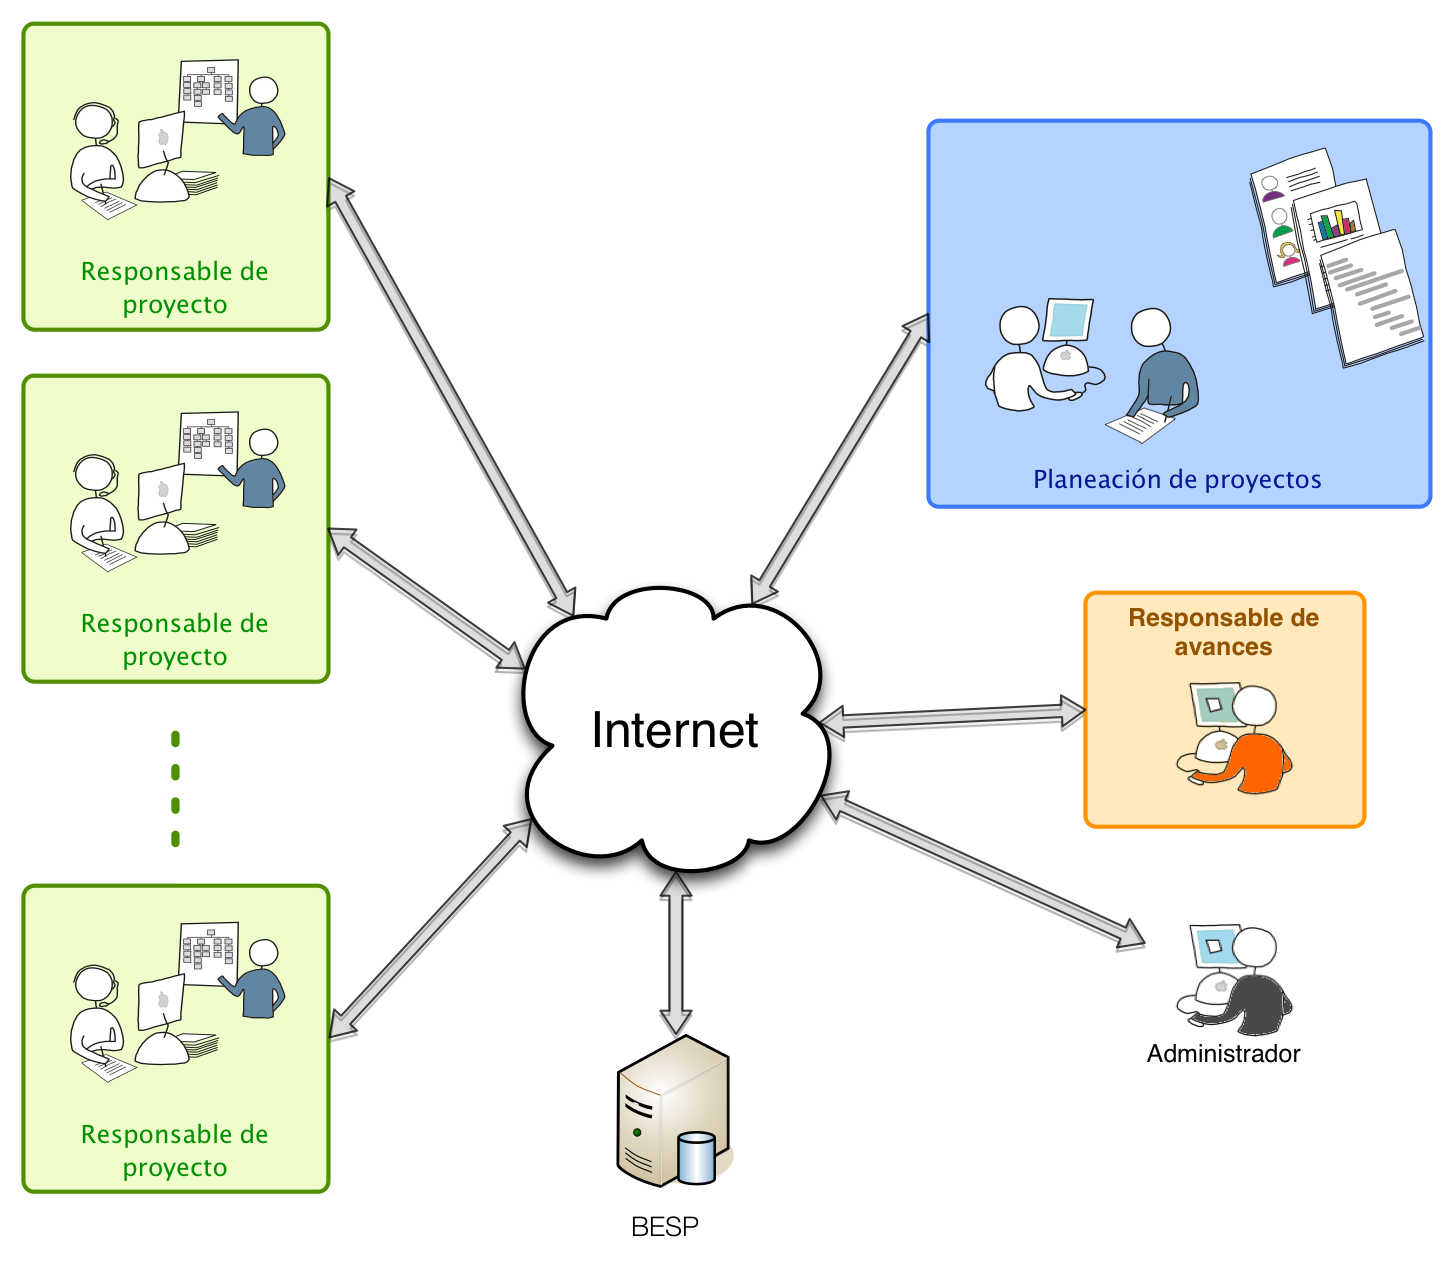
\includegraphics[width=.7\textwidth]{images/arquitectura}}
		\caption{Arquitectura del sistema.}
		\label{fig:arquitectura}
	\end{center}
\end{figure}

En la figura~\ref{fig:arquitectura} se describe la estructura del sistema, en ella se detalla ...

